\section{Problèmes au cours du projet}

\subsection{Modification des Scripts}

Dans un premier temps, nous avons créé des premières pages HTML afin d'avoir un rendu visuel et de définir un premier style CSS servant à voir, pour le développement, à quoi s'apparenterait les pages finales.

\begin{figure}[H]
    \begin{center}
	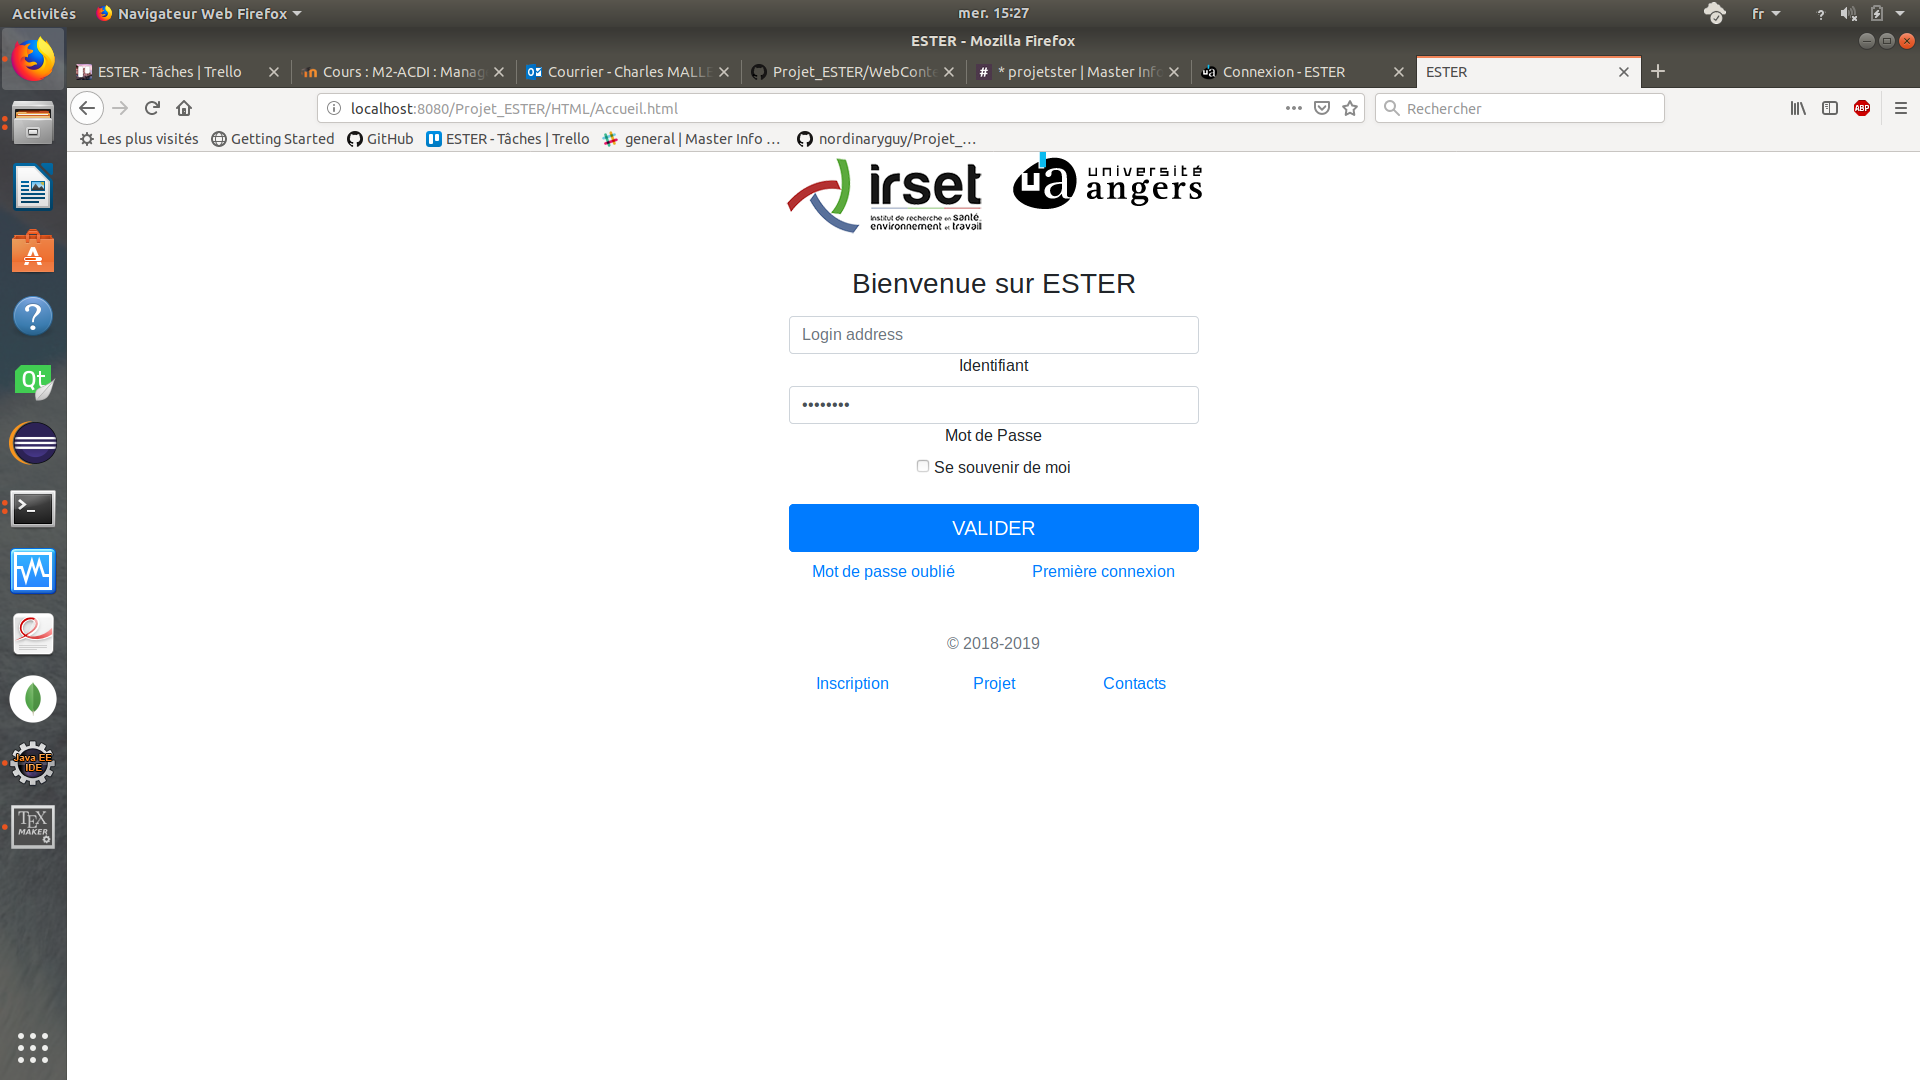
\includegraphics[scale=0.2,trim=4cm 0cm 4cm 5.3cm, clip=true]{img/OldConnexion}
    \end{center}
    \caption{Ancienne Page de Connexion}
\end{figure}

\begin{figure}[H]
    \begin{center}
	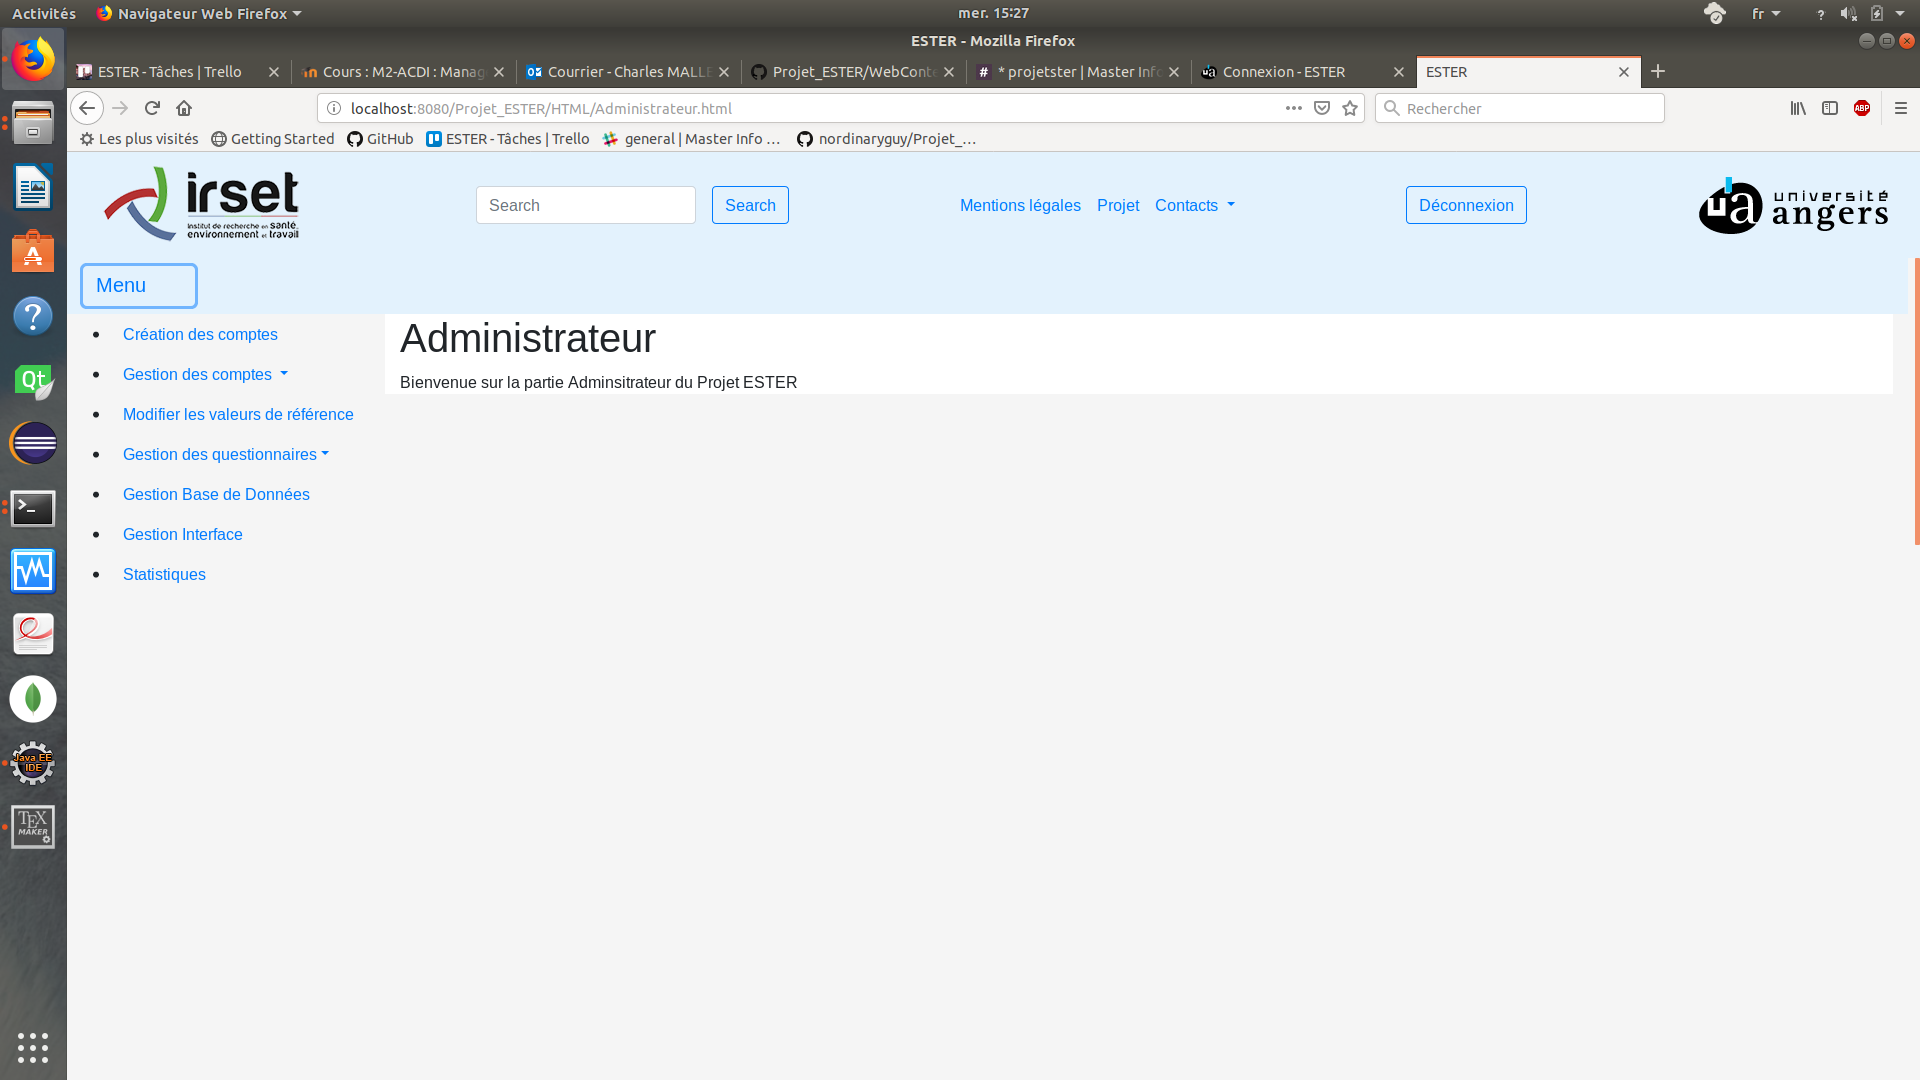
\includegraphics[scale=0.2,trim=2.8cm 0cm 0.8cm 5.3cm, clip=true]{img/OldAdmin}
    \end{center}
    \caption{Ancienne Page de l'Administrateur}
\end{figure}

Au sein de nos pages, nous avons défini des liens permettant d'appeler des pop-up de Bootstrap. Ces Modals devaient nous permettre d'une manière élégante de créer des comptes ou encore d'appeler la partie de modification de l'interface utilisateur par l'administrateur.

\begin{figure}[H]
    \begin{center}
	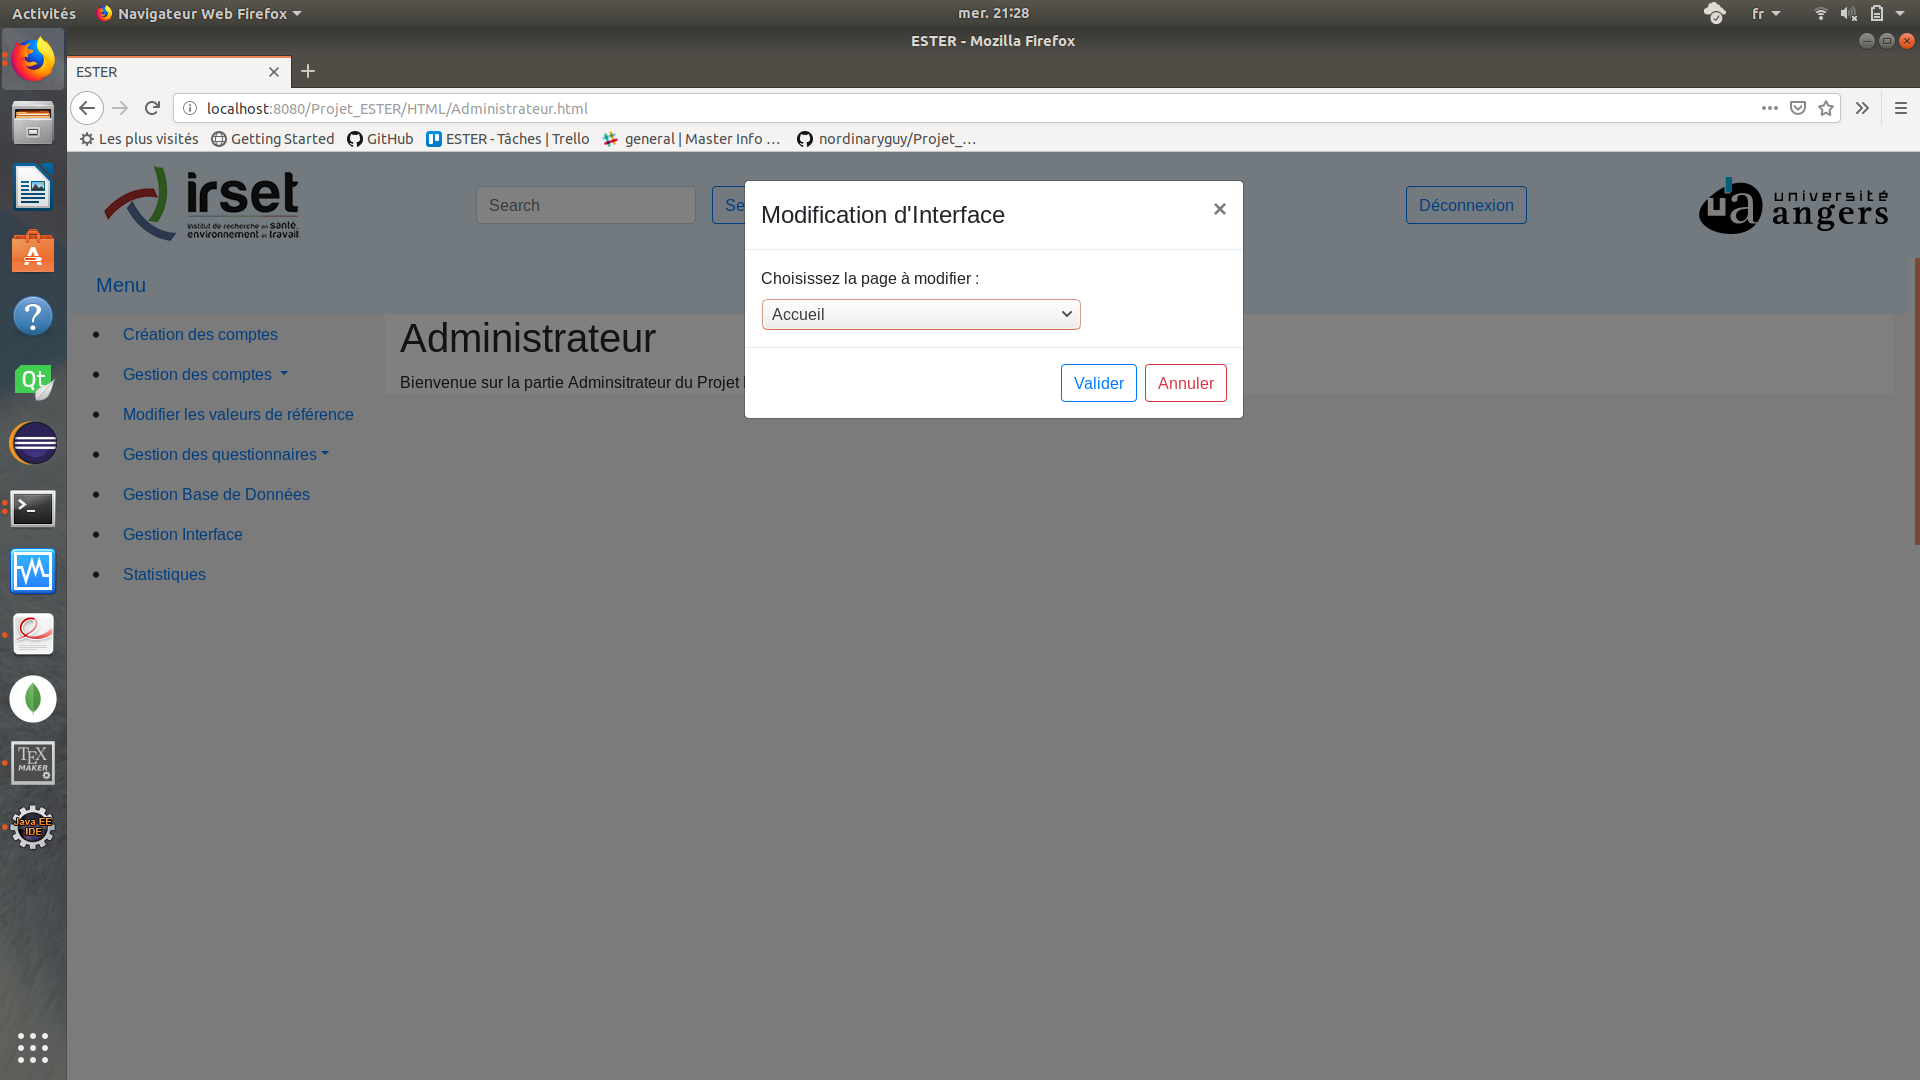
\includegraphics[scale=0.2,trim=2.8cm 0cm 0.8cm 5.3cm, clip=true]{img/modal}
    \end{center}
    \caption{Modal avec Bootstrap}
\end{figure}

L'interface de modification graphique permettait à l'administrateur de modifier à loisir chaque page du site comme il le souhaitait. Grâce à JQuery, nous récupérions la page choisie dans un modal et l'interface permettait de faire glisser de nouveaux éléments dans la page selon le désir de son utilisateur. Il pouvait également les supprimer ou les redimensionnés, tout en demeurant responsive.

\begin{figure}[H]
    \begin{center}
	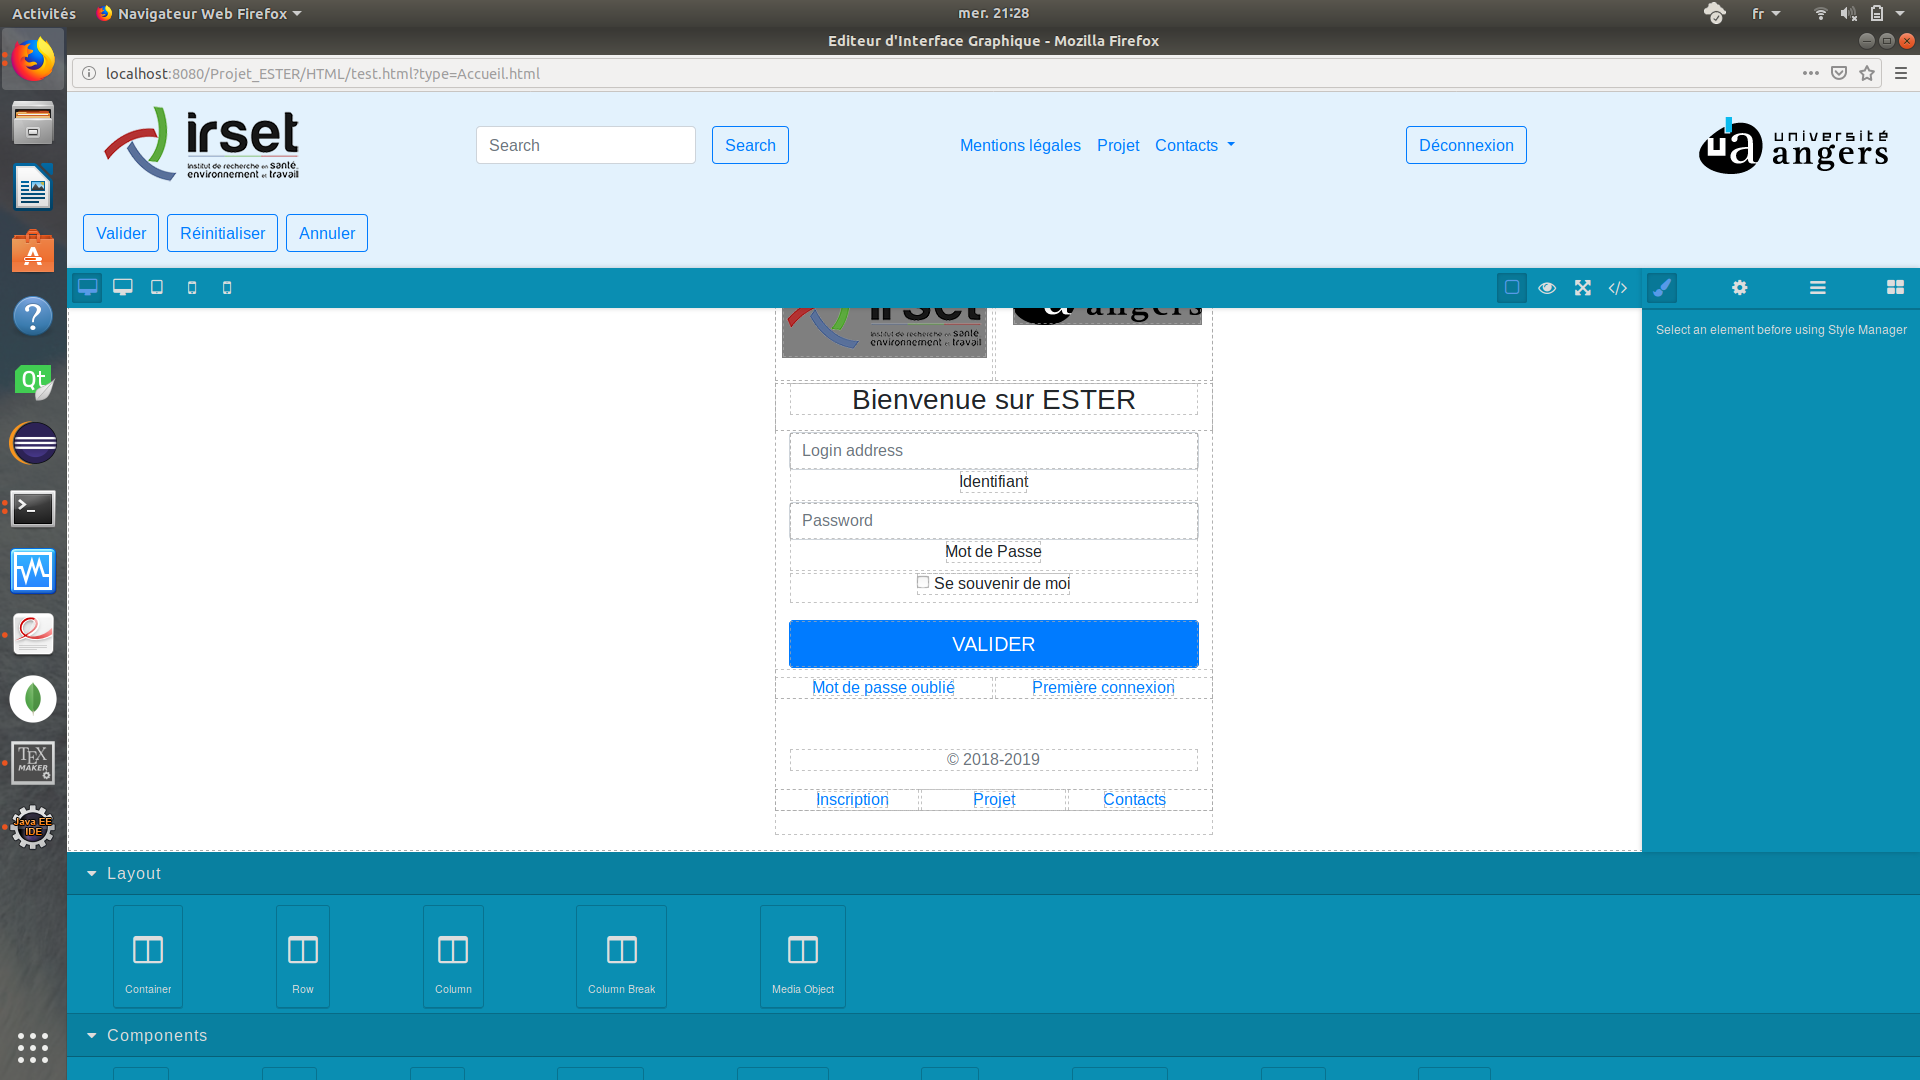
\includegraphics[scale=0.2,trim=2.8cm 0cm 0.8cm 4.0cm, clip=true]{img/interface}
    \end{center}
    \caption{Interface de modification graphique pour l'administrateur}
\end{figure}


Toutefois, les scripts HTML ont fini remplacés par des scripts JSP car plus avantageux comme dit précédemment. De ce fait, les modals et l'interface utilisateur, n'étant plus compatibles avec les nouveaux scripts, ont été laissés. D'un autre côté, nous n'avons pas tous défini de la même manière nos styles CSS. Ce fut les membres d'ESTER qui décidèrent au cours de la réunion de novembre du visuel qu'ils préféraient. Nous avons ensuite appliqués les modifications voulues et directement réécrit dans des scripts JSP. Cependant, ces changements nous ont coûté un peu de temps qui aurait pu nous être utile dans l'implémentation d'autres fonctionnalités.

\subsection{Versions Bootstrap et JQuery}

N'étant pas tous parti de la même origine, d'un même code, nous avons développé chacun nos tâches à part tel que nos chefs de projet nous les donnaient. Cependant, lors de l'intégration commune en novembre, nous nous sommes aperçus de certaines incompatibilités. Certaines parties étaient développés avec la dernière version de Bootstrap et la dernière de JQuery, tandis que d'autres utilisaient la précédente. 
De ce fait, il fut plus compliqué, plus laborieux de réunir chaque partie et de faire correspondre chaque page à nos propres normes. 


\section{Perspectives d'amélioration}

Malgré les nombreuses semaines à travailler sur ce projet, nous n'avons pas été en mesure de finir totalement le projet. Avec les difficultés listées précédemment et les tâches de plus en plus nombreuses, nous n'avons pu que faire au mieux. 
Le projet que nous avons à vous proposer correspond donc avant tout aux principales fonctionnalités attendues. Toutefois, il serait envisageable d'intégrer davantage les entreprises dans le site puisqu'elles sont légèrement délaissées. 
Également, les questionnaires créés par les médecins et administrateurs ne prennent pas en compte les scores qui seraient grandement utiles dans les calculs des statistiques. 
Nous pouvons penser qu'à terme, il serait remis l'interface de modification graphique. Bien qu'elle fut avant tout penser en HTML, il devrait être possible de la réutiliser en correspondance avec le JSP. 
